A partir de la unidad anterior podemos obtener una familia de algoritmos que se basa en el uso de cadenas de Markov. Estos se llaman \textbf{Markov Chain Monte Carlo} y tienen variadas aplicaciones, incluyendo optimización global de funciones no convexas.

\newp Algunos de los casos de uso incluyen situaciones en las que uno no necesariamente desea llegar a un óptimo global sino más bien un buen mínimo local. Pese a esto, en algunos casos existen garantías de convergencia y son competitivos con métodos deterministas.

\newp Referencias en Pardoux \cite{pardoux} y Metropolis, N., Rosenbluth, A. W., Rosenbluth, M. N., Teller, A. H., Teller, E.  \cite{metro}.
\subsection{Cadenas de Markov reversibles} % clase 12 lunes 5 oct
\begin{proposition}
\label{prop:4_1_1}
Sea $\xcm\sim\cm$, $n\in\N$ entonces $(\hat{X}_n)_{n=0}^N:=(X_{N-n})_{n=0}^N$ es cadena de Markov \textbf{no homogénea} con
$$ \P(\hat{X}_{n+1}=y|\hat{X}_n=x)=\displaystyle\frac{(\mu P^{N-n-1})_y}{(\mu P^N)_x}P_{yx} \, .$$
En particular si $\mu=\pi$ con $\pi$ distribución invariante de $P$, donde $P$ es irreducible, entonces $(\hat{X}_n)_{n=0}^N$ es $CM(\pi,\hat{P})$ homogénea con matriz de transición:
$$ \hat{P}_{xy}=\displaystyle\frac{\pi_y}{\pi_x}P_{yx} \, .$$
\end{proposition}
\begin{proof}
\gris
\begin{alignat*}{2}
    \P(\xhat_{n+1}=y|\xhat_{n}=X_n,\dots,\xhat_0=x_0) & = \displaystyle \frac{\P_\mu(X_N=x_0,\dots,X_{N-n}=x_n,X_{N-n-1}=y)}{\P_\mu(X_N=x_0,\dots,X_{N-n}=x_n)} \\
     & = \frac{(\mu P^{N-n-1})_yP_{y,x_n}P_{x_n,x_{n-1}},\dots,P_{x_0,x_0}}{(\mu P^{N-n})_{x_n}P_{y,x_n}P_{x_n,x_{n-1}},\dots,P_{x_1,x_0}} \\
     & =  \frac{(\mu P^{N-n-1})_yP_{y,x_n}}{(\mu P^{N-n})_{x_n}} = \frac{\P_\mu(X_{N-n-1}=y,X_{N-n}=x_n)}{\P_\mu(X_{N-n}=x_n)}\\
     & = \P(\hat{X}_{n+1}=y|\hat{X}_n=x_n) \, .
\end{alignat*}
\findem
\negro 
\end{proof}
\begin{definition}[Reversibilidad]
Sea $\xcm$ cadena de Markov irreducible recurrente positiva en equilibrio. Decimos que es reversible si $\forall n\in\N$
$$ Ley((X_n)_{n=0}^N)=Ley((X_{N-n})_{n=0}^N)\espacio(=Ley((\hat{X}_{n})_{n=0}^N)) \, .$$
\end{definition}
\begin{proposition}[Condición de balance detallado]
Sea $\xcm$ cadena de Markov irreducible recurrente positiva en equilibrio. $X$ es \textbf{reversible} si y sólo si $(\pi,P)$ cumplen la condición de balance detallado:
$$ \pi_xP_{xy}=\pi_yP_{yx}\forall x,y\in E\, .$$
\end{proposition}
\begin{proof}
\gris
\mbox{ }\newline ($\Rightarrow$) Reversible $\implies \P_\pi(X_0=x,X_1=y)(=\pi_xP_{xy})=P_\pi(X_1=x,X_0=y)(=\pi_yP_{yx})$
\newline ($\Leftarrow$) \mbox{Balance detallado } $\implies \hat{P}_{xy}:=\displaystyle\frac{\pi_y}{\pi_x}P_{yx}=P_{xy}$
\newline $\therefore (\hat{X}_n)_{n=0}^N\sim CM(\pi,P)$ gracias a la proposición \ref{prop:4_1_1}. \findem
\negro
\end{proof}
% \vspace{.5cm}\\
\begin{remark}
\beforeitemize
\begin{itemize}
    \item Notación: si $(\pi,P)$ están en balance detallado, decimos también que $\pi$ es reversible con respecto a $P$ y vice-versa.
    \item Si tenemos $P$ matriz estocástica irreducible y $\pi\in\mathcal{P}(E)$ es reversible (i.e., en balance detallado) con respecto a $P$,  entonces $\pi$ es invariante para $P$. En efecto: 
    $$ \pi_xP_{xy}=\pi_yP_{yx}\implies (\pi P)_y=\pi_y (\mbox{ sumando para }x\in E)\, .$$
    La recíproca no es cierta en general.
    \item $\pi$ es reversible con respecto a $P$ si y solo si  $$\P_\pi(X_{n+1}=y,X_n=x)=\P_\pi(X_{n+1}=x,X_n=y)\espacio \forall x, y \in E \,.$$
    \item $\pi$ es invariante con respecto a $P$ si y solo si % $\ssi$  
    $$\forall y \in E,\espacio \P_\pi(X_{n+1}=y,X_n\neq y)=\P_\pi(X_{n+1}\neq y,X_n\neq y)\,.$$
\end{itemize}
\end{remark}
\begin{example}[Grafo no-orientado finito]
Sea $G$ grafo no-orientado finito. Sea $(X_n)_{n\in\N}$ un paseo aleatorio simple, es decir: 
$$ P_{xy}=\P(X_{n+1}|X_n=x):=\begin{cases}
\frac{1}{deg_x}   & \mbox{ si }y\sim x\\
0   & \mbox{ si no,}
\end{cases}$$
con $deg_x=|\{y|y\sim x\}|$ (i.e., el grado de cada vértice). Entonces
$$ deg_x\cdot P_{xy}=1=deg_y \cdot P_{yx}, \forall x,y$$
$$ \therefore \pi=(\pi_x)_{x\in E}=\displaystyle\bigg(\frac{deg_x}{\sum_{y\in E}deg_y}\bigg)_{x\in E} \mbox{ está en balance detallado con }P \, .$$
$$ \therefore \pi \mbox{ es invariante.}$$
\end{example}
\subsection{Markov Chain Monte Carlo}
\subsubsection{Idea general}
Sea $\pi\in \mathcal{P}(E),\pi>0$
\newline \textbf{Pregunta: ¿existe $P$ matriz estocástica (irreducible) tal que $\pi P=\pi$?} ($\pi$ invariante con respecto a $P$).
\newp La utilidad de esto sería que si queremos \textbf{simular} aproximadamente una variable aleatoria $x_\infty\sim\pi$, basta encontrar $P$ tal que $\pi P=\pi$ y simular $(X_n)_{n\in\N}\sim \cm$ por tiempo suficiente.
\newline \textbf{Es más fácil buscar $P$ matriz estocástica tal que $\pi_xP_{xy}=\pi_yP_{yx} \mbox{ (reversible) }, \forall x.y\in E$}\,.

\newp \textbf{Objetivo}: dado $\pi\in\mathcal{P}(E),\pi>0$, queremos construir $P$ irreducible tal que $(\pi,P)$ estén en balance detallado y tal que $(X_n)_{n\in\N}\sim CM(\mu,P)$ es fácilmente simulable.
\subsubsection{Los métodos MCMC}
Partimos con $R=(R_{xy})_{xy\in E}$ matriz de transición irreducible ``cualquiera'' tal que $\forall x,y$,\\ $R_{xy}>0\implies R_{yx}>0$ y además, cuyas transiciones (de $CM(\pi,R)$) sean fáciles de simular.
\newline Luego definimos
$$ P_{xy}=\begin{cases}
\min(R_{xy},(\frac{\pi_y}{\pi_x})R_{yx})  & \mbox{ si }x\neq y\\
1-\displaystyle\sum_{z\neq x}P_{xz}  & \mbox{ si }x=y
\end{cases}$$
\begin{proposition}
$P=(P_{xy})$ es matriz estocástica irreducible y $(\pi,P)$ están en balance detallado.
\end{proposition}
\begin{proof}
\gris
\beforeitemize
\begin{itemize}
    \item Veamos que es matriz estocástica: $\sum_{y\neq x}p_{xy}\leq \sum_{y\neq x}R_{xy}\leq 1 \implies P_{xx}\in[0,1]$ y $\sum_z P_{xz}=1$.
    \item Para la irreducibilidad notemos que $\forall x,y\in E$ existen $n,x_1,\dots,x_n\in E$ tal que 
    $$R_{xx_1},R_{x_2,x_3},\dots,R_{x_ny}>0\,,$$
    luego $R_{yx_n},R_{x_n,x_{n-1}},\dots,R_{x_1y}>0$, con lo cual $P_{xx_1},\dots,P_{x_ny}>0$.
    \item El caso $x=x$ es directo. Para $x\neq y$, $\pi_xP_{xy}=\pi_xR_{xy}\land \pi_yR_{yx}=\pi_yP_{yx}$. \\ Entonces se tiene la condición de balance detallado.
\end{itemize}
\findem
\negro
\end{proof}

\newp \textbf{¿Cómo escoger $R$?}
\newline Elegimos un grafo no orientado $G$ con conjunto de vértices $E$ y  $R$ tal que $\forall x,y$, $R_{xy}>0$ si y sólo si $x \sim y$ (vecino) en $G$.
\newline Dos elecciones ``clásicas'' son:
\begin{itemize}
    \item \textbf{Gibbs sampler} (muestreo de Gibbs)
    $$ R_{xy}=\begin{cases}
    \pi_{y}(\displaystyle\sum_{z\sim x}\pi_z)^{-1}  & \mbox{ si }x\sim y\\
    0  & \mbox{ si no}
    \end{cases}$$
    \item \textbf{Algoritmo metrópolis} (paseo aleatorio simple en $G$)
    $$ R_{xy}=\begin{cases}
    \displaystyle\frac{1}{deg_x} & \mbox{ si }x\sim y\mbox{ con }deg_x=|\{y:y\sim x\}|\\
    0  & \mbox{ si no}
    \end{cases}$$
\end{itemize}
\subsubsubsection{Metropolis-Hasting}
\label{m-h}
\textbf{¿Cómo simular $(X_n)_{n\in\N}\sim CM(\mu,P)$?}
\newline Sean $(V_n)_{n\in\N}\sim\iid \unif$ y $f:[0,1]\times E\to E$ función de transición asociada a $R$.
\newline Sean $(U_n)_{n\geq 1}\sim \iid\unif$ independientes de las $(V_n)_{n\in\N}$. Simulamos $X_0=Y_0\sim\mu$ usando $V_0$.
\newline Luego, recursivamente definimos:
\begin{itemize}
    \item Dado $X_n=x$, simulamos
    $$ Y_{n+1}:=f(V_{n+1},x)=y \mbox{, es decir, una transición según }R\,.$$
    \item Definimos
    $$ X_{n+1}=\begin{cases}
    Y_{n+1}  & \mbox{ si } \espacio U_{n+1}\leq \displaystyle\frac{\pi_y R_{yx}}{\pi_x R_{xy}}  \\
    X_n  & \mbox{ si } \espacio U_{n+1}> \displaystyle\frac{\pi_y R_{yx}}{\pi_x R_{xy}}
    \end{cases}$$
\end{itemize}
\begin{proposition}
$$ (X_n)_{n\in\N}\sim CM(\mu,P)$$
\end{proposition}
\begin{proof}
\gris
$\forall x\neq y$ tenemos:
\begin{alignat*}{2}
    \P(\xhat_{n+1}=y,\xhat_{n}=y) & = \P\bigg(f(V_{n+1},x)=y,X_n=x,U_{n+1}\leq \displaystyle\frac{\pi_y R_{yx}}{\pi_x R_{xy}}\bigg) \\
     & = R_{xy}\P\bigg(U_{n+1}\leq \frac{\pi_y R_{yx}}{\pi_x R_{xy}}\bigg)\P(X_n=x)\\
     & = R_{xy}\min\bigg(\frac{\pi_y R_{yx}}{\pi_x R_{xy}},1\bigg)\P(X_n=x) \,,
\end{alignat*}
$\implies \P(X_{n+1}=y| X_n=x)=\displaystyle\min\{\frac{\pi_y}{\pi_x}R_{yx},R_{xy}\}=P_{xy}$\,,
\newline y $\P(\xhat_{n+1}=y|\xhat_{n}=x)=1-\displaystyle\sum_{y\neq x}\P(X_{n+1}=y|X_n=x)=1-\sum_{y\neq x}P_{xy}=P_{xx}$\,. \findem
\negro
\end{proof}
\begin{remark}
La construcción sólo requiere conocer $\lambda = \alpha \pi$ con $\alpha>0$ una constante (depende sólo de $\displaystyle \frac{\pi_x}{\pi_y},x$ e $y$). % \newline 
Esto es muy importante en la práctica pues muchas veces se conoce sólo la medida $\lambda$ en $E$, y calcular la constante de normalización puede ser inviable numéricamente si $E$ es grande.
\end{remark}
% \vspace{.5cm} \\ %%%%%%%%%%
\begin{remark}
El grafo $G$ debe escogerse idealmente de forma que
\begin{itemize}
    \item No haya estados ``muy aislados'', de modo que una $CM(\mu,R)$ lo ``recorre bien'' y $(X_n)_{n\in\N}\sim CM(\mu,P)$ ``alcanza rápido'' el equilibrio.
    \item Las transiciones desde cada $x$ sean fáciles de simular (lo que es m\'as difícil si $x$ tiene demasiados vecinos).
\end{itemize}
Notar que estas dos propiedades apuntan  en sentidos contrarios.
\end{remark}
\vspace{.5cm} \\ %%%%%%%%%%
\begin{remark}  % clase 13 7 oct
En el caso Gibbs,  para calcular $(R_{xy})_{xy\in E}$, hay que calcular sumas $\sum_{z\sim x}\pi_z$, $x\in E$\,.
    \newline \underline{Atención}: si $x$ tiene muchos vecinos, calcular estas sumas puede ser impracticable. Entonces es mejor usar Metropolis.
\end{remark}
\subsection{Aplicación de MCMC: simulated annealing}
%\subsubsection{Simulated Annealing}
Simmulated annealing (``recocido simulado'') tiene como objetivo \textbf{minimizar} una funci\'on o  ``energía'' $U:E\to\R$ (donde $E$ es grande) con un algoritmo estocástico.
\newp Consideramos un par\'ametro  $\beta>0$ que denominamos ``temperatura inversa'' (i.e., $T=\beta^{-1}$ representa la temperatura).
\vspace{.2cm} \\ %%%%%%%%%%
\begin{definition}[Medida de Gibbs]
Definimos $\pi^\beta\in\mathcal{P}(E)$ mediante:
$$ \pi^\beta_x = \displaystyle \frac{\exp^{-\beta U(x)}}{Z_\beta}\,,$$
con
$$ Z_\beta = \displaystyle\sum_{y\in E}\exp^{-\beta U(y)} \espacio\mbox{constate de normalización}\,.$$
A $\pi^\beta$ se le llama medida de Gibbs.
\vspace{.5cm} \\ %%%%%%%%%%
\end{definition}
\begin{remark}
\beforeitemize
\begin{itemize}
    \item $\pi^\beta$ da más probabilidad a los $x$ con menor $U(x)$\,.
    \item Cuando $\beta \searrow 0$ ($T\nearrow\infty$): $\pi^\beta\mbox{ }\substack{\longrightarrow \\ \beta\to\infty}\mbox{ }Unif(E)$\,,
    i.e., es indiferente de la energia $U$\,.
    \item ¿Que pasa cuando $\beta\nearrow \infty$ ($T\searrow 0$)?
    \newline Sean $U_*=\min U$, $A_U=\arg\min U$,
    \begin{alignat*}{2}
        \pi^\beta_x & = \displaystyle\frac{e^{-\beta U(x)}}{\sum_{y\inA_U}e^{-\beta U(y)}+\sum_{y\in A^C_U}e^{-\beta U(y)}} \\
         & = \displaystyle\frac{e^{-\beta U(x)}}{\# A_U e^{-\beta U_*}+\sum_{y\in A^C_U}e^{-\beta U(y)}} \\
         & = \displaystyle\frac{e^{-\beta (U(x)-U_*)}}{\# A_U +\sum_{y\in A^C_U}e^{-\beta (U(y)-U_*)}}) \mbox{ }\substack{\longrightarrow \\ \beta\to\infty}\mbox{ }\begin{cases}
    \frac{1}{\# A_U}  & \mbox{ si } x\in A_U  \\
    0  & \mbox{ si } x \notin A_U
    \end{cases}
    \end{alignat*}
    Entonces si $\beta\nearrow \infty$,\espacio $\pi^\beta\mbox{ }\substack{\longrightarrow \\ \beta\to\infty}\mbox{ }\pi^\infty=Unif(A_U)$\,.
    \item Para cada $\beta>0$ sabemos simular $(X^\beta_n)_{n\in\N}$ (reversible) que converge en ley a $\pi^\beta\propto e^{-\beta U}$ cuando $n\to\infty$\,.
\end{itemize}
\end{remark}
La idea del método \textbf{Simmulated annealing} consiste en tomar $\beta_n\searrow \infty$ y simular una cadena de markov no homogénea $\xcm$``$=$''$(X_n^{\beta_n})_{n\in\N}$ (usando Metropolis-Hastings (\ref{m-h})), es decir, en cada tiempo $n$, simular transición tal que
$$ \P(X_{n+1}=y|X_n=x)=\P(X_{n+1}^{\beta_{n+1}}=y|X_n^{\beta_{n+1}}=x)\,.$$
\vspace{.5cm}\\
Antes de estudiar como hacerlo, veamos qu\'e hace $(X^\beta_n)_{n\in\N}$ cadena simulada con Metropolis-Hastings con $\beta>0$ fijo.
\begin{itemize}
    \item Contamos con $G$ grafo \underline{regular} no orientado con conjunto de v\'ertices $E$\,.
    \item $\pi^\beta \propto e^{-\beta U(x)}, \forall x \in E$\,.
    \item En el tiempo $n$, dado que $X_n=x$, simulamos
    $ y=Y_{n+1}\sim Unif\{z:z\sim x\}$, transición desde $x$ para un paseo aleatorio simple ($R_{xy}=(deg(G))^{-1}, \forall x\sim y$)\,.
    \item Sampleamos $U_{n+1}\sim\unif \indep$ de todo y 
    $$ X_{n+1}^\beta =\begin{cases}
    Y_{n+1}=y  & \mbox{ si } U_{n+1}\leq\displaystyle\min\bigg\{\displaystyle\frac{\pi_y^\beta}{\pi_x^\beta},1\bigg\} , \\
    X_n^\beta  & \mbox{ si } U_{n+1}>\min\bigg\{\displaystyle\frac{\pi_y^\beta}{\pi_x^\beta},1\bigg\}\espacio.
    \end{cases}$$
    Notemos que  $\min\bigg\{\displaystyle\frac{\pi_y^\beta}{\pi_x^\beta},1\bigg\} = \min \{ e^{-\beta(U(y)-U(x))},1\}$. Luego: 
    \begin{itemize}
        \item Si $U(y)<U(x)$ la transición siempre se realiza pues  el m\'inimo es $1$ y $U_{n+1}\leq 1$ siempre. Esto quiere decir que si la energía del estado propuesto $y$ es menor que la del estado actual $x$, la transición se realiza de todos modos.
        \item Si $U(y)\geq U(x)$  el m\'inimo es menor que $1$, luego se realiza la transici\'on si  $U_{n+1}\leq e^{-\beta(U(y)-U(x))}$, y en caso contrario ($>$) no. As\'i, si la propuesta es transitar a un estado de mayor energía, esto puede llevarse acabo a veces,  pues puede permitir salir de un mínimo local, distinto del mínimo  global buscado.
    \end{itemize}
\end{itemize}
Entonces,  si $\beta\gg 1 $ ($0<T\ll  1 $) el valor de la energ\'ia es menos propenso a ``subir'' en cada paso, y \textbf{tiende a ir hacia un m\'inimo}  (que puede no ser global). Por otro lado si $0<\beta\ll  1$ ($T\gg 1$),  la energ\'ia fluct\'ua de manera más aleatoria, pudiendo  subir o bajar en cada paso, lo que permite \textbf{escapar de mínimos locales}.
\newp Así, para $n$ pequeño ($\beta_n$ pequeño y $T_n$ alta), $X_n$ tiende a pasearse por todo $E$ sin tomar muy en cuenta el ''paisaje de energ\'ia'' dado por $U$ (desorden), mientras que, para $n$ grande ($\beta_n$ grande y $T_n$ chico) $X_n$ se mueve muy poco, sólo alrededor de algún mínimo (local) hasta que se ``congela'' ahí. 

El  siguiente resultado indica una elecci\'on  te\'orica para $\beta_n$ que asegura convergencia a m\'inimos globales: 


\begin{theorem}
Sea $$\triangle >Osc(U):=\displaystyle\max_{x\in E}U(x)-\min_{x\in E}U(x)\,.$$
Entonces, si $\beta_n:=\displaystyle\frac{1}{\triangle}\log(1-n)$
$$ \implies Ley(X_n)\conv\pi^\infty=Unif(A_U) \mbox{ minimizante}\,.$$
Más aún, se prueba que $X_n\convp A_U$ (mínimo global).
\end{theorem}
\begin{proof}
\gris
Ver Pardoux cap 10 \cite{pardoux} para una versión para C.M. en tiempo continuo. 
\negro
\end{proof}
% \vspace{1cm} \\ %%%%%%%%%%
\begin{remark}
\beforeitemize
\begin{itemize}
    \item En la práctica $\ln(1+n)$ es demasiado lento para poder observar una evoluci\'on descendiente de la energ\'ia.
    \item Usualmente se suele escoger:
    \begin{itemize}
        \item $\beta_n$ polinomial en $n$ (por ejemplo $n^2$)
        \item $\beta_n$ exponencial en $n$, 
    \end{itemize}
    pero no hay garantías de convergencia a $A_U$ en esos casos.
    \item En cada problema hay que jugar con distintas sucesiones $(\beta_n)_{n\in\N}$ tal que $\beta_n\nearrow \infty$\, y puntos de inicio $X_0$, y escoger finalmente el mejor m\'inimo encontrado. 
    \item El algoritmo da una heurística para encontrar buenos mínimos locales más eficiente que optimización discreta.
\end{itemize}
\end{remark}
\textbf{Idea física}:
\newline ``Annealing'' = recocido, viene de la metalurgia y se refiere a un  procedimiento para hacer más dúctil (menos duro) una aleación, calentando(a) por sobre el nivel de cristalización y dejándola enfriar lentamente para alcanzar un estado de energía potencial basal material homogéneo, pocas ``dislocaciones''.
\newline Si el enfriamiento es muy rápido queda un material homogéneo pero duro:
\newline ``Quenching''=templado.
\begin{figure}
    \centering
    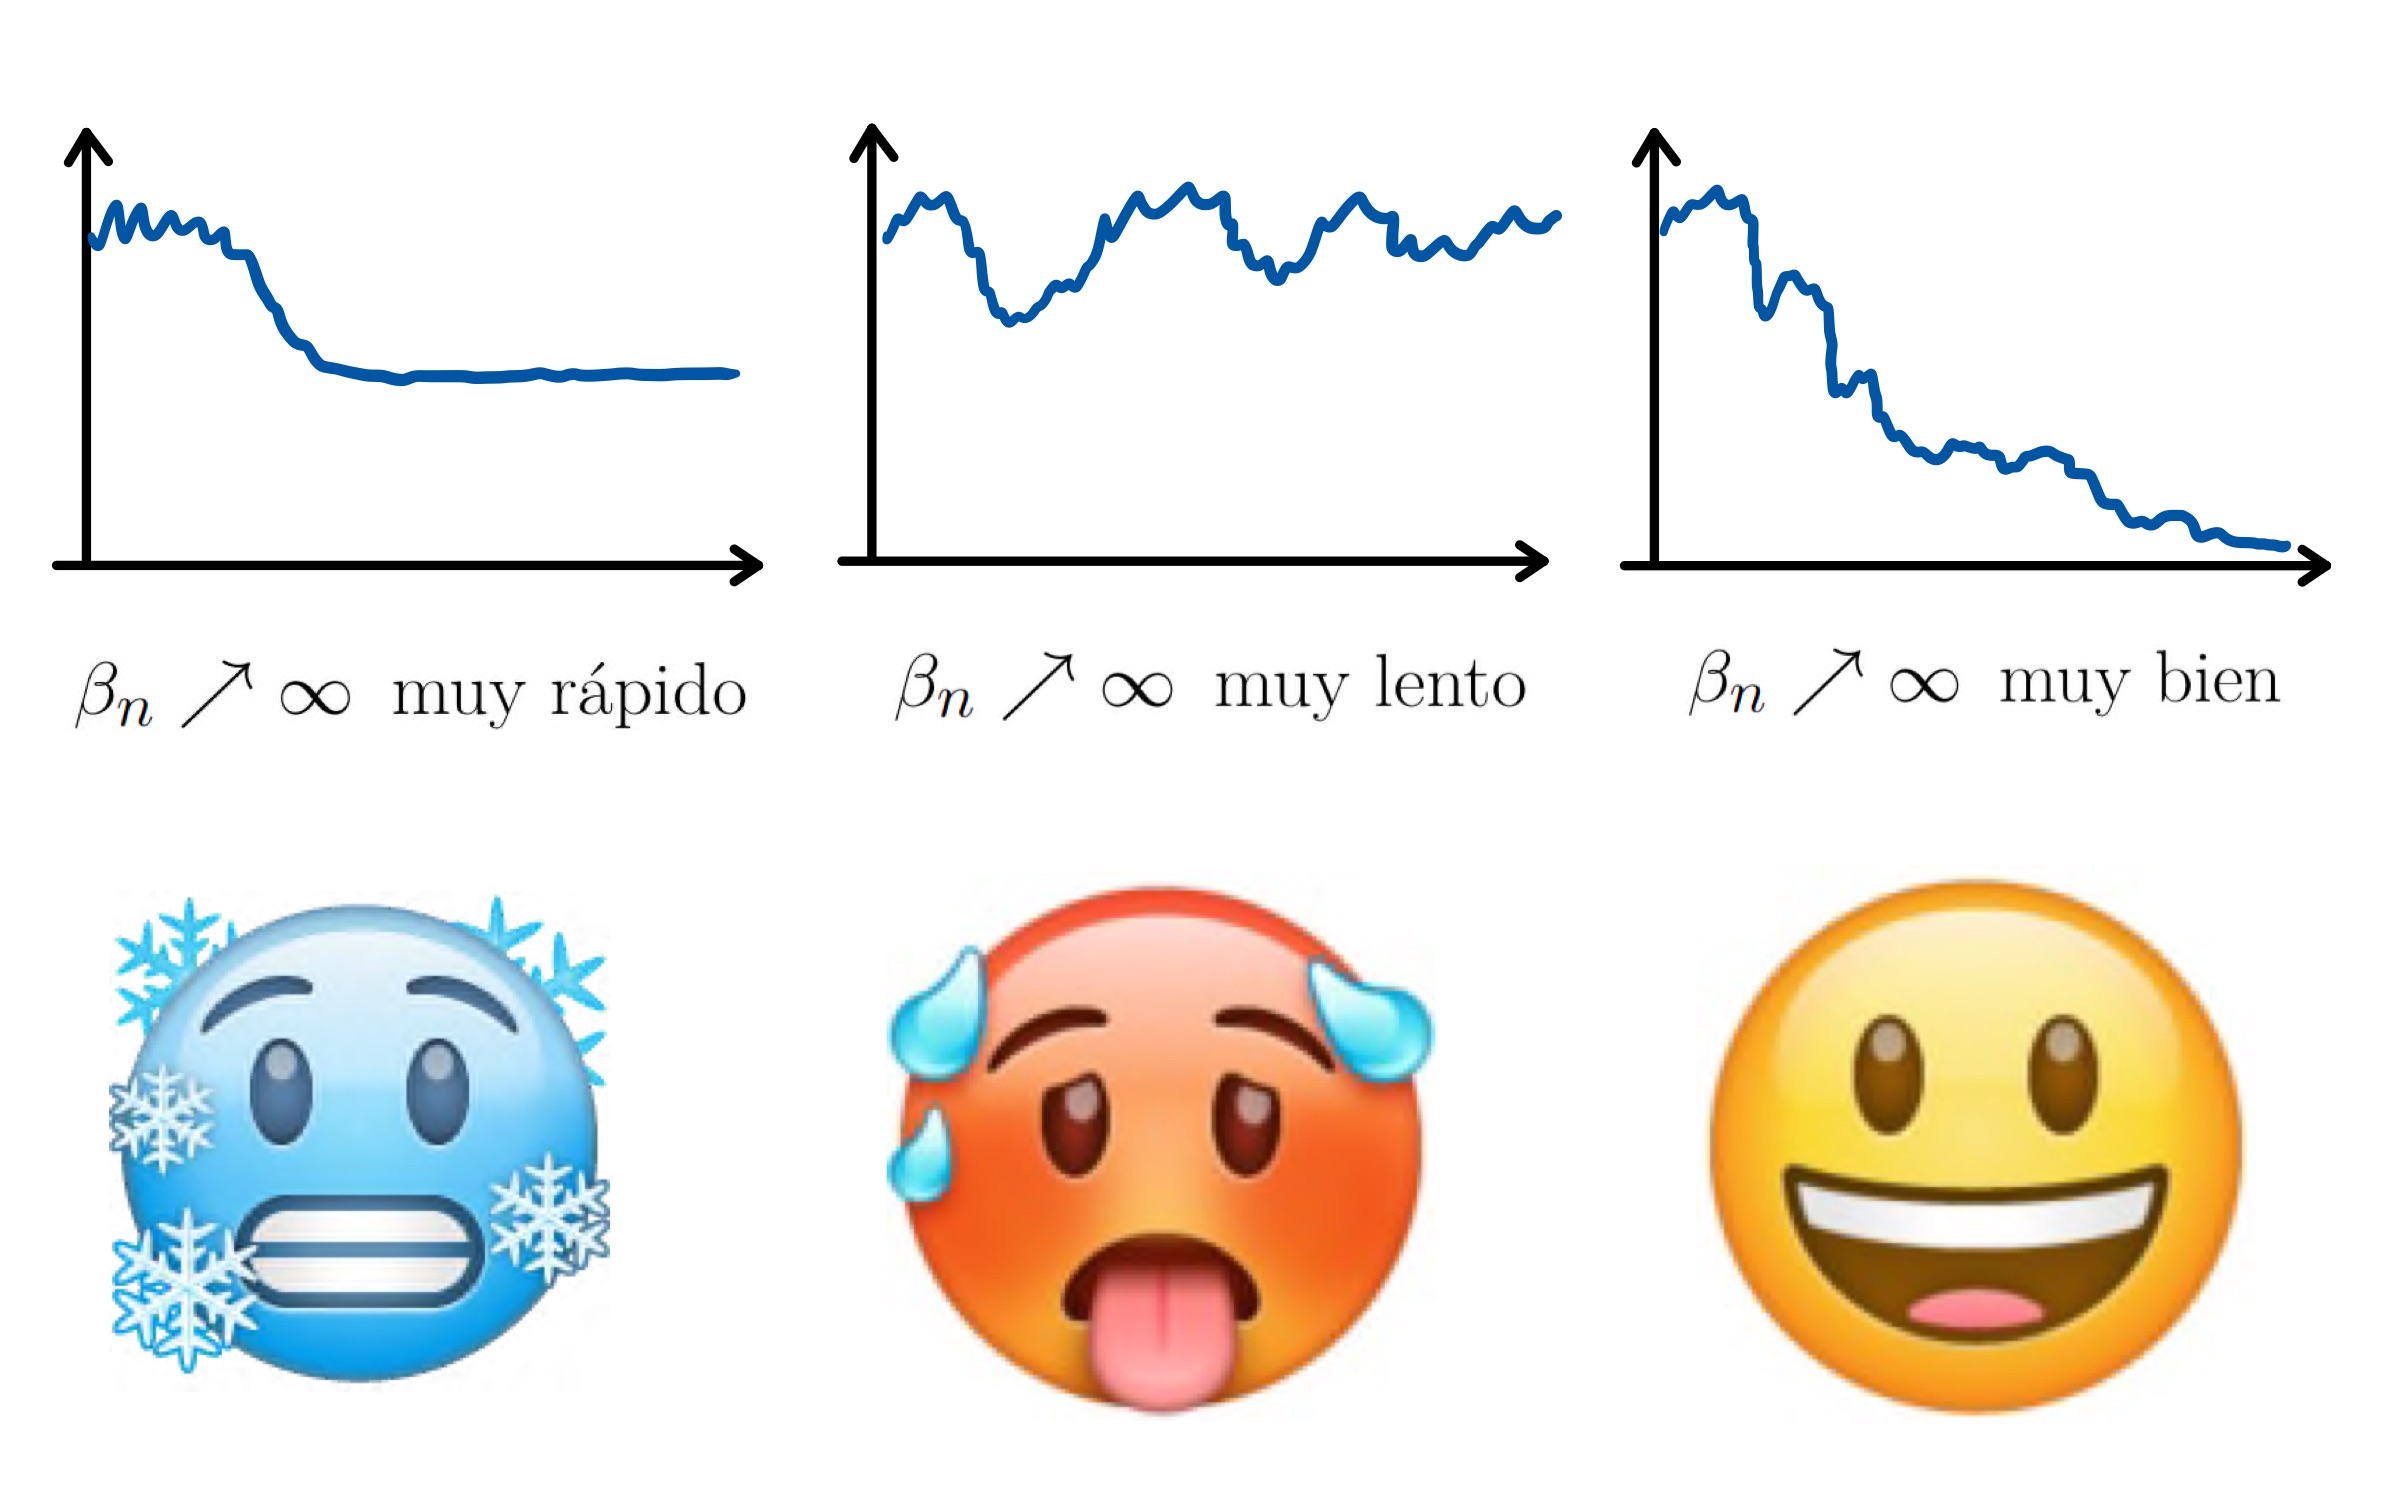
\includegraphics[scale=0.16]{img/clase_14_pag_12.jpg}
    \caption{Idea del efecto de las sucesiones $\beta_n$ en la minimización de la energía $U$.}
    \label{fig:betas}
\end{figure}

% \newpage
\subsection{MCMC y estadística Bayesiana}
\subsubsection{Recuerdo de estadística Bayesiana}
\textbf{Idea}: modelamos simultaneamente y probabilisticamente:
\begin{itemize}
    \item Observaciones $x$ de un fenómeno o dato aleatorio, cuya ley ``$p(x|\theta)$'' depende de un parámetro $\theta\in\Theta$.
    \item La incertidumbre, desconocimiento o conocimiento parcial de $\theta$, lo que representamos asumiendo que $\theta$ es aleatorio y sólo conocemos su distribución ``$p(\theta)$'' ``a priori''.
    \item En lo anterior, la observación $x$ está en un conjunto $\mathfrak{X}$ que puede ser subconjunto de $\R^d$, un conjunto finito o numerable, etc. 
    \newline En general $x\mapsto p(x|\theta)$ (ley de $x$ dado $\theta$) es
    \begin{itemize}
        \item o bien una función de masa discreta: 
        $$\displaystyle\sum_{x\in \mathfrak{X}}p(x|\theta)=1$$
        \item o bien una densidad de probabilidad: 
        $$\displaystyle\int_{\mathfrak{X}}p(x|\theta)dx=1\,.$$
    \end{itemize}
    \item $x$ puede ser una ``muestra'' $x=(x_1,\dots,x_n)$.
    \item $\Theta$ puede ser subconjunto de $\R^k$, conjunto finito o numerable y $p(\theta)$ denota, seg\'un corresponda:
    \begin{itemize}
        \item una función de masa discreta
        \item o bien una densidad de probabilidad,
    \end{itemize}
    con respecto a $\theta$,  y se le llama \textbf{ley a priori}.
    \item $p(x,\theta):=p(x|\theta)p(\theta)$ es ley conjunta en $\mathfrak{X}\times \Theta$ del parámetro y una observación.
    \newline Notar que
    $$ \displaystyle\int_\Theta\int_\mathfrak{X} p(x,\theta)dxd\theta=\int_\Theta\int_\mathfrak{X} p(x|\theta)dx p(\theta)d\theta=1\,.$$
    \item Dado $\theta\in\Theta$, $x\mapsto p(x|\theta)$ se llama ley de $x$ dado $\theta$, o bien la densidad de $x$ condicional a $\theta$.
    \item Dado $X\in\mathfrak{X}$ observación, $\theta\mapsto L(\theta)=L_X(\theta)=p(X|\theta)$ se llama \textbf{función de verosimilitud} (likelihood). Notar que $\int L(\theta)d\theta\neq1$ en general.
\end{itemize}
\textbf{Objetivo de la inferencia Bayesiana}: ``Re-estimar'' el parámetro $\theta$ (modificar o actualizar la ley que describe lo que sabemos de $\theta$) usando la información que nos da el observar $x$.
\begin{theorem}[Bayes]
La ley de $\theta$ dado $x$, también llamada ley posterior de $\theta$, está dada por:
\begin{alignat*}{2}
    p(\theta|x) & := \displaystyle \frac{p(x,\theta)}{p(x)}\\
     & = \displaystyle\frac{p(x|\theta)p(\theta)}{p(x)} \,,
\end{alignat*}
con $p(x)=\displaystyle\int_\Theta p(x,\theta)d\theta$ ley marginal (no condicional).


\end{theorem}
Luego $p(\theta|x)\propto p(x|\theta)p(\theta)$. De esta forma,   $p(x)$ aparece  sólo como una constante de normalización, dependiente de la observaci\'on $x$, cuyo c\'alculo requiere en general sumar o integrar sobre todo el espacio. Por ello,    \textbf{calcular la constante de normalizaci\'on  $p(x)$ puede ser muy costoso,   y hay  evitar tener que hacerlo}.  Es por este motivo que los m\'etodos MCMC son muy \'utiles en este contexto, como veremos un poco m\'as adelante. 
\subsubsection{Aplicaciones de estadística Bayesiana}
\begin{itemize}
    \item Observamos $x_!,\dots,x^n \iid \sim p(x|\theta)dx$ con $\theta$ fijo.
    \newline Sean $\mathcal{D}=\{x_1,\dots,x_n\}$ ``datos'' y su densidad conjunta dada por:
    $$ p(\mathcal{D}|\theta):=p(x_1,\dots,x_n|\theta)=\displaystyle\prod^n_{i=1}p(x_i|\theta)\, . $$
    Además,  consideramos su función de verosimilitud:
    $$ L_\mathcal{D}(\theta)=L_{x_1,\dots,x_n}(\theta)=\displaystyle\prod^n_{i=1}L_{x_i}(\theta)$$
    \item Luego la ley a posteriori de $\theta$ dados $\mathcal{D}$ es la ley en $\Theta$: $$\mathcal{D}=p(\theta|x_1,\dots,x_n)=\displaystyle\frac{\prod^n_{i=1}p(x_i|\theta)p(\theta)}{p(\mathcal{D})}\propto \prod^n_{i=1}p(x_i|\theta)p(\theta)\,$$
    donde la última expresión es evaluable.  $p(\mathcal{D})$ es la densidad marginal de los datos y requiere integrar:
    $$ \displaystyle \int_\Theta p(\mathcal{D}|\theta)p(\theta)d\theta=\int_\Theta\prod^n_{i=1}p(x_i|\theta)p(\theta)d\theta\,.$$
    \item En base a $p(\theta|\mathcal{D})=p(\theta|x_1,\dots,x_n)$, finalmente se construye un ``\textbf{posterior predictivo}'', i.e., un valor $\hat{\theta}_n\in\Theta$ (``estimador de $\theta$'') que mejor explica los datos $x_1,\dots,x_n$.
\end{itemize}
\vspace{1cm}\\
\subsubsubsection{Ejemplos de estimadores Bayesianos}
Los siguiente son estimadores Bayesianos clásicos (hay muchos otros):
\begin{itemize}
    \item \textbf{Media a posteriori}
    \newline Considera  como estimador predictivo la media con respecto a la ley a posteriori de $\theta$.
    $$ \hat{\theta}_n = \displaystyle\int_\Theta p(\theta|\mathcal{D})d\theta\,.$$
    \item \textbf{Máximo a posteriori}
    \newline Es un par\'ametro cuyo  valor  maximiza la probabilidad a posteriori de observar la data $\mathcal{D}$
    \begin{alignat*}{2}
        \hat{\theta}_n & := \displaystyle\arg\max_{\theta} p(\theta|\mathcal{D})\\
         & = \arg\max_{\theta}[\sum^n_{i=1}\log p(x_i|\theta)+\log p(\theta)]\,.
    \end{alignat*}
    En la práctica, la maximización se lleva a cabo como en la última expresión.
\end{itemize}
\begin{remark}
\beforeitemize
\begin{itemize}
    \item También es posible construir regiones o \textbf{regiones o intervalos de confianza} para $\theta$, es decir (para $\theta$ real), un intervalo $I$ tal que $\P(\theta\in I | X_1,\dots,X_n)\approx 95\%$ (por ejemplo).
    \item Se requiere ``conocer'' $p(\theta|\mathcal{D})$ para optimizar en $\theta$ o bien para integrar $p(\theta|\mathcal{D})$ con respecto a $\theta$. En algunos (pocos) casos, $p(\theta|\mathcal{D})$ tiene forma analítica explícita.
\end{itemize}
\end{remark}
%\begin{example}
%\beforeitemize
%\begin{itemize}
%    \item Una moneda... %clase 15 min 48 pag8-9
%\end{itemize}
%\end{example}
\subsubsection{Uso de MCMC}
En general $p(\theta|x_1,\dots,x_n)=\displaystyle \prod^n_{i=1}p(x_i|\theta)p(\theta)$ no tiene forma cerrada.
\newline Además para tener su valor numérico, se requiere integrar $\int\prod^n_{i=1}p(x_i|\theta)p(\theta)d\theta=p(x_1,\dots,x_n)$, lo cual puede ser muy costoso.
\newp \textbf{Idea}: samplear de
\begin{alignat*}{2}
    \Pi(\theta) & := p(\theta|x_1,\dots,x_n)\\
     & = \displaystyle \frac{\prod^n_{i=1}p(x_i|\theta)p(\theta)}{p(\mathcal{D})}\,
\end{alignat*}
usando MCMC en $\Theta$, pues con este m\'etodo \textbf{no se requiere conocer ni calcular $p(\mathcal{D})$, y 
basta poder evaluar rápidamente $\prod^n_{i=1}p(x_i|\theta)p(\theta)$}. La cadena de Markov construida con MCMC vive en $\Theta$ y tiene distribución invariante $$\Pi(\theta)\propto\displaystyle\prod^n_{i=1}p(x_i|\theta)p(\theta)\,.$$  
Cabe notar que: 
\begin{itemize}
    \item el m\'etodo puede aplicarse tanto para $\Theta$ discreto como $\Theta=\R^k$ (usando ``paseo aleatorio en $\R^k$ como cadena Markov de base''). %algo más pag 11
    \item la simulación es costosa en general, sobretodo si el espacio de parámetros tiene dimensión muy grande (se requiere correr muchas veces la cadena de MCMC, por mucho tiempo).
\end{itemize}
